\documentclass[]{article}

\usepackage{tikz}
\usepackage{amsmath}
\usepackage{amsfonts}
\usepackage{amssymb}
\usepackage{tkz-base}
\usepackage{tkz-euclide}
\usepackage{xcolor}
\usepackage{pgfplots}
\usepackage{graphicx}
\usepackage{url}
\usepackage{mathptmx}
\usepackage[american,siunitx]{circuitikz}
\usepackage{pgfplots}
\usepackage{cancel}
\usepackage{tabularray}

% Required packagef
\usetikzlibrary{positioning}
\usetikzlibrary{svg.path}
\usetikzlibrary{arrows}
\usetikzlibrary{shapes.geometric,calc}
\usetikzlibrary{calc,arrows.meta,backgrounds}
\usetikzlibrary{shapes, positioning, patterns, decorations, decorations.markings}
\usetikzlibrary{decorations.pathreplacing}

\newcommand{\mymotor}[2] % #1 = name , #2 = rotation angle
{\draw[thick,rotate=#2] (#1) circle (10pt)
    node[]{$\mathsf M$} 
    ++(-12pt,3pt)--++(0,-6pt) --++(2.5pt,0) ++(-2.8pt,6pt)-- ++(2.5pt,0pt);
    \draw[thick,rotate=#2] (#1) ++(12pt,3pt)--++(0,-6pt) --++(-2.5pt,0) ++(2.8pt,6pt)-- ++(-2.5pt,0pt);
}

\newdimen\XCoord
\newdimen\YCoord
\newcommand*{\ExtractCoordinate}[1]{\path (#1); \pgfgetlastxy{\XCoord}{\YCoord};}%

\newcommand{\gear}[3]{%
  \def\modu{#1}
  \def\Zb{#2}
  \def\AngleA{#3}

  \pgfmathsetmacro{\Rpr}{\Zb*\modu/2}
  \pgfmathsetmacro{\Rb}{\Rpr*cos(\AngleA)}
  \pgfmathsetmacro{\Rt}{\Rpr+\modu}
  \pgfmathsetmacro{\Rp}{\Rpr-1.25*\modu}
  \pgfmathsetmacro{\AngleT}{pi/180*acos(\Rb/\Rt)}
  \pgfmathsetmacro{\AnglePr}{pi/180*acos(\Rb/\Rpr)}
  \pgfmathsetmacro{\demiAngle}{180/\Zb}
  \pgfmathsetmacro{\Angledecal}{(\demiAngle-2*\AnglePr)/2}

  \foreach \zz in{1,2,...,\Zb}{
    \draw
    ({(\zz))/\Zb*360-\Angledecal}:\Rb)
    -- (\zz/\Zb*360-\Angledecal:\Rp)
    to[bend right=\demiAngle]
    (\zz/\Zb*360+\Angledecal:\Rp)
    --
    plot[domain=-0:\AngleT,smooth,variable=\t]
    ({{180/pi*(-\t+tan(180/pi*\t)) +\zz/\Zb*360+\Angledecal}:\Rb/cos(180/pi*\t)})
    % 
    to[bend right=\demiAngle]
    ({{180/pi*(\AngleT+tan(180/pi*-\AngleT)) +(\zz+1)/\Zb*360-\Angledecal}:
      \Rb/cos(180/pi*-\AngleT)})
    % 
    plot[domain=-\AngleT:-0,smooth,variable=\t]
    ({{180/pi*(-\t+tan(180/pi*\t)) +(\zz+1)/\Zb*360-\Angledecal}:\Rb/cos(180/pi*\t)});
  }
}


%opening
\title{Modeling and Control of a Single Joint}
\author{Craig Carignan \& Glen Henshaw}

\begin{document}
\maketitle

\section{Intro}
We're going to talk about how to model (and, maybe, control) the dynamics of a single joint at the actuator level. This will include the dynamics of an electric motor, any gear--based transmission, joint flexibility, and friction. We're going to skip the modeling of linear actuators (electric or otherwise) because in practice rotational motion via electric motors covers 99\% of what we see in practice. Note that some robotic arms are hydraulic, specifically arms designed to work in the subsea; the modeling and control of hydraulic actuators is its own thing that we could easily spend an entire class (or at least a couple of lectures) talking about. For more info on hydraulic actuation and control, see the excellent textbook \textit{Hydraulic Control Systems} by Noah Manning and Roger Fales (John Wiley \& Sons 2019). Pneumatic actuator control, which is also sometimes used, is even more complex than hydraulic control due to the compressibility of air (or whatever other gas you might consider using). As a consequence, accurate high bandwidth control of pneumatics is very much an open research problem.

\section{Electric Motor}
Here's a cross section of a simple brushed DC motor:
\begin{figure}[h!]
	\centering
            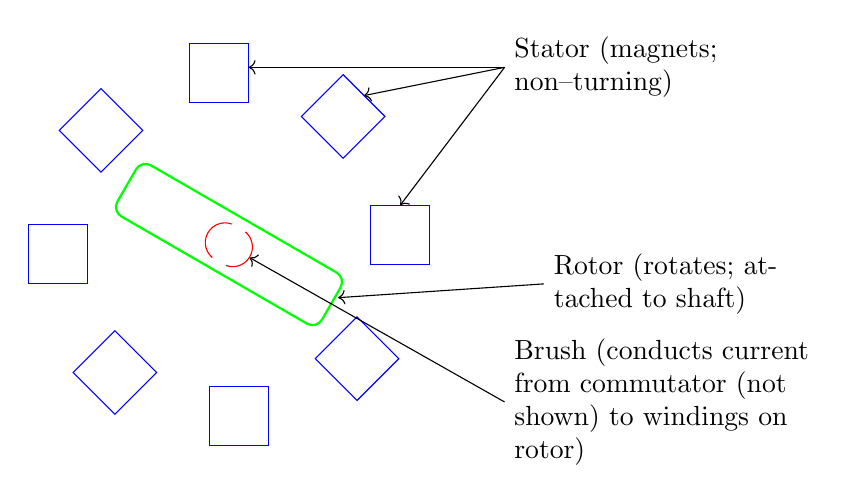
\begin{tikzpicture}
            	%\draw[thick] (0,0) circle (3cm);
            	\foreach \r in {0, 45, 90, 135, 180, 225, 270, 315} {
            		 \draw [color=blue, rotate=\r] (-0.5, 1.8) rectangle +(0.75,0.75) coordinate (m_\r);
            	}
            	\draw[color=green, thick, rounded corners] [rotate=-30] (-1.5, -0.375) rectangle +(3,0.75) coordinate (rotor);
		\draw[color=black, <-] (rotor)++(-0.1, -0.25) -- (4, -0.5) node[right, text width=3cm] {Rotor (rotates; attached to shaft)};
		\draw[color=black, <-] (m_0)++(0, -0.3) -- (3.5, 2.25) node[right,  text width=3cm] {Stator (magnets; non--turning)};
		\draw[color=black, <-] (m_315)++(0.707*-0.375,0.707*0.375) -- (3.5, 2.25);
		\draw[color=black, <-] (m_270)++(-0.375,0.75) -- (3.5, 2.25);
		\draw[color=red] [rotate=-30] (0.1,-0.25cm) coordinate (brush) arc [start angle = -80, end angle = 80, radius = 0.25cm] (-0.1,-0.25cm) arc [start angle = -100, end angle = -260, radius = 0.25cm];
		\draw[color=black, <-] (brush)++(0.3, 0.1) -- (3.5, -2) node[right,  text width=4cm]{Brush (conducts current from commutator (not shown) to windings on rotor)};
            \end{tikzpicture}
\end{figure}

\noindent
Typically, the torque produced by a motor like this varies sinusoidally as the angle of the rotor moves with respect to the fixed stator magnets; this is called ``torque ripple''. For a decent motor the torque ripple will be perhaps 5\% of the average torque.

\noindent
The physics that allow a motor to generate a torque are described by:
\begin{displaymath}
	F = qV \times B
\end{displaymath}
where a charge $q$ moving through a magnetic field $B$ with velocity $V$ experiences a force $F$. The charges are the electrons moving through the windings in the rotor, and the magnetic field is generated by the (usually permanent) magnets in the stator. Usually, the torque of a motor is related to the current flowing through the windings via the ``motor torque constant'':
\begin{equation}
	\tau_{m} = K_{m}I_{a} \label{torqueconstant}
\end{equation}
As we might recall from a few lectures ago, the torque constant isn't actually a constant -- so this is very definitely an approximation.

\noindent
When a motor is moving, it acts as a generator and it develops a voltage across its armature. A second motor constant called the ``back emf constant'' describes the generated voltage as a function of rotational velocity:
\begin{equation}
	V = K_{e}\dot{\theta}_{M} \label{emfconstant}
\end{equation}
Here is the electrical circuit of a motor:
\begin{figure}[h!]
	\centering
    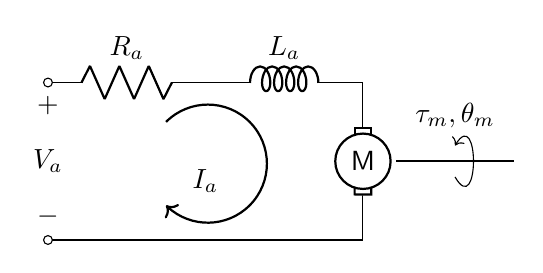
\begin{tikzpicture}[damper/.style={thick,
            decorate,
            decoration={markings,  
                mark connection node=dmp,
                mark=at position 0.5 with 
                {
                    \node (dmp) [thick, inner sep=0pt, 
                    transform shape, 
                    rotate=-90, 
                    minimum width=15pt, 
                    minimum height=10pt, draw=none] {};
                    \draw [thick] ($(dmp.north east)+(4pt,0)$) -- 
                    (dmp.south east) -- (dmp.south west) -- 
                    ($(dmp.north west)+(4pt,0)$);
                    \draw [thick] ($(dmp.north)+(0,-8pt)$) -- 
                    ($(dmp.north)+(0,8pt)$);
        }}},]

        \draw (0,2) to[R=$R_a$,o-] ++(2,0)  to[L,cute inductor, l=$L_a$,]  ++(2,0)  to[sV, color=white, name=M1] ++(0,-2) to[short,-o] ++(-4,0);
        \mymotor{M1}{90}
        \draw (0,2) to [open, v=$V_a$] (0,0);
        \draw[thick] (M1.north) -- ++(1.5,0);% -- +(0,0.5) node [anchor=south] {$N_1$} -- +(0,-0.5) coordinate (N1);
                \draw[->] ([xshift=7.5mm,yshift=-2mm]M1.north)  to [out=-60,in=60, looseness=4] ++(0,0.4) node [above=1mm] {$\tau_m, \theta_m$};
        \draw[thick, ->] (1.5,1.5) arc [start angle = 135, end angle = -135, radius = 0.75];
        \draw (2, 0.75) node {$I_a$};
    \end{tikzpicture}
    \label{motor_circuit}
\end{figure}

\noindent
where $L_{a}$ is the armature inductance, $R_{a}$ is the armature resistance, and $V_{a}$ is the voltage. The dynamics of this circuit are:
\begin{displaymath}
	L_{a}\dot{I}_{a} + R_{a}I_{a} = V_{a} - K_{e}\dot{\theta}_{M}
\end{displaymath}
If we assume that the inductance of the circuit is negligible, this ceases to be a differential equation and we can derive a ``torque--speed'' curve as follows:
\begin{displaymath}
	V_{a} = R_{a}I_{a} + K_{e}\dot{\theta}_{m}
\end{displaymath}
and we can substitute Equation \ref{torqueconstant} for $i_{a}$ and then solve for $\tau_{m}$ to get
\begin{displaymath}
	\tau_{M} = \frac{K_{m}}{ R_{a}}\left(V_{a} - K_{e}\dot{\theta}_{M}\right)
\end{displaymath}

\pagebreak
\noindent
Plotting this, we get:
\begin{figure}[h!]
    \centering
    \begin{tikzpicture}
        \begin{axis}[
            ticks=none,
            axis lines = left,	
            xlabel = $\tau_m$,
            ylabel = $\dot{\theta}$
        ]
        \addplot[color=red]{-5*x+3};
        \end{axis}
        \draw (1.25,6) node {unloaded speed = $\frac{V_{a}}{K_{e}}$};
        \draw (8.5,0) node {stall torque = $\frac{K_{m}V_{a}}{R_{a}}$};
	\draw (3.8, 3) node {\rotatebox{-40}{$V_{a}=\ $constant}};
    \end{tikzpicture}
    \caption{A torque--speed curve}
\end{figure}
\section{Transmission}
Motors are (almost) always high speed, low torque devices (i.e. the unloaded speed of a small electric motor will generally be in the range of 500-2000 RPMs). Robots ``want'' high torque and low speed. Traditionally, we use a transmission to trade speed for torque.
\noindent
Here's a simplified drawing of a geartrain transmission:
\begin{figure}[h!]
	\centering
	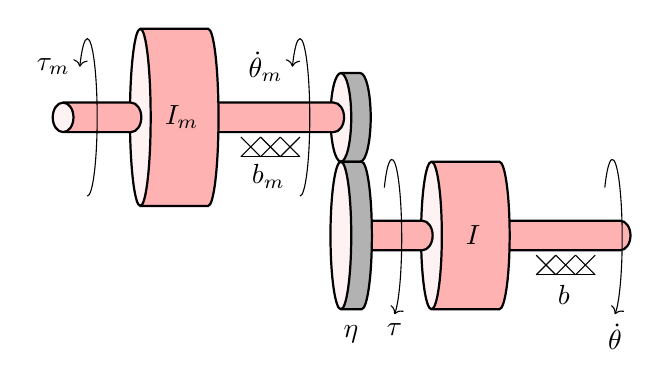
\begin{tikzpicture}
		\coordinate(A) at (0cm,0cm);
		\coordinate(B) at (5cm, 0cm);
		\coordinate(C) at ($ (A)!1.25cm!(B) $);
		\coordinate(D) at ($ (A)!-0.95cm!(B) $);
		\coordinate(E) at ($ (C)!1cm!(B) $);
		\coordinate(F) at ($(E)!1.5cm!-90:(B) $);
		\coordinate(G) at ($(F)+(3.75cm,0cm)$);
		\coordinate(H) at ($(F)!0.5cm!(G)$);
		\coordinate(I) at ($(H)!0.95cm!(G)$);
		\coordinate(J) at ($(I)!1cm!(G)$);
		
		\draw (E) node[cylinder,draw=black,thick,aspect=1.5,minimum height=0.5cm,minimum width=1.5cm,rotate=180,cylinder uses custom fill, cylinder body fill=black!30,cylinder end fill=red!5,scale=0.75]{};
		\draw (C) node[cylinder,draw=black,thick,aspect=1.5,minimum height=2.5cm,minimum width=0.5cm,rotate=180,cylinder uses custom fill, cylinder body fill=red!30,cylinder end fill=red!5,scale=0.75]{};
		\draw (A) node[cylinder,draw=black,thick,aspect=1.5,minimum height=1.5cm,minimum width=3cm, rotate=180,cylinder uses custom fill, cylinder body fill=red!30,cylinder end fill=red!5,scale=0.75]{};
		\draw (D) node[cylinder,draw=black,thick,aspect=1.5,minimum height=1.5cm,minimum width=0.5cm,rotate=180,cylinder uses custom fill, cylinder body fill=red!30,cylinder end fill=red!5,scale=0.75]{};
		
		\draw (J) node[cylinder,draw=black,thick,aspect=1.5,minimum height=3cm,minimum width=0.5cm,rotate=180,cylinder uses custom fill, cylinder body fill=red!30,cylinder end fill=red!5,scale=0.75]{};
		\draw (I) node[cylinder,draw=black,thick,aspect=1.5,minimum height=1.5cm,minimum width=2.5cm,rotate=180,cylinder uses custom fill, cylinder body fill=red!30,cylinder end fill=red!5,scale=0.75]{};
		\draw (H) node[cylinder,draw=black,thick,aspect=1.5,minimum height=1.5cm,minimum width=0.5cm,rotate=180,cylinder uses custom fill, cylinder body fill=red!30,cylinder end fill=red!5,scale=0.75]{};
		\draw (F) node[cylinder,draw=black,thick,aspect=1.5,minimum height=0.5cm,minimum width=2.5cm,rotate=180,cylinder uses custom fill, cylinder body fill=black!30,cylinder end fill=red!5,scale=0.75]{};
		
		% Draw crosshatch "dampers"
		\draw ($(E)-(1.5cm, 0.5cm)$) -- ($(E)-(1.25cm, 0.25cm)$);
		\draw ($(E)-(1.5cm, 0.25cm)$) -- ($(E)-(1.25cm, 0.5cm)$);
		\draw ($(E)-(1.25cm, 0.5cm)$) -- ($(E)-(1cm, 0.25cm)$);
		\draw ($(E)-(1.25cm, 0.25cm)$) -- ($(E)-(1cm, 0.5cm)$);
		\draw ($(E)-(1cm, 0.5cm)$) -- ($(E)-(0.75cm, 0.25cm)$);
		\draw ($(E)-(1cm, 0.25cm)$) -- ($(E)-(0.75cm, 0.5cm)$);
		\draw ($(E)-(1.5cm, 0.5cm)$) -- ($(E)-(0.75cm, 0.5cm)$);
		\draw ($(E)-(1.15cm, 0.75cm)$) node {$b_m$};
		
		\draw ($(G)-(1.5cm, 0.5cm)$) -- ($(G)-(1.25cm, 0.25cm)$);
		\draw ($(G)-(1.5cm, 0.25cm)$) -- ($(G)-(1.25cm, 0.5cm)$);
		\draw ($(G)-(1.25cm, 0.5cm)$) -- ($(G)-(1cm, 0.25cm)$);
		\draw ($(G)-(1.25cm, 0.25cm)$) -- ($(G)-(1cm, 0.5cm)$);
		\draw ($(G)-(1cm, 0.5cm)$) -- ($(G)-(0.75cm, 0.25cm)$);
		\draw ($(G)-(1cm, 0.25cm)$) -- ($(G)-(0.75cm, 0.5cm)$);
		\draw ($(G)-(1.5cm, 0.5cm)$) -- ($(G)-(0.75cm, 0.5cm)$);
		\draw ($(G)-(1.15cm, 0.75cm)$) node {$b$};

		\draw ($(F)-(0.1cm, 1.25cm)$) node {$\eta$};
		
		\draw [->] ($(D)-(0.25cm, 1cm)$) arc [start angle=-90, end angle=140, x radius=0.125cm, y radius=1cm] node [left] {$\tau_m$};
		\draw [->] ($(E)-(0.75cm, 1cm)$) arc [start angle=-90, end angle=140, x radius=0.125cm, y radius=1cm] node [left] {$\dot{\theta}_m$};
		\draw [<-] ($(I)-(1cm, 1cm)$) node [below] {$\tau$} arc [start angle=-75, end angle=140, x radius=0.125cm, y radius=1cm];
		\draw [<-] ($(G)-(0.5cm, 1cm)$) node [below] {$\dot{\theta}$} arc [start angle=-75, end angle=140, x radius=0.125cm, y radius=1cm];
		\draw (A) node {$I_m$};
		\draw (I) node {$I$};
	\end{tikzpicture}
\end{figure}

\noindent
where the gear ratio, $\eta$, is greater than 1 (often, considerably greater; gear ratios of 500 aren't uncommon, and the FREND arms used on the RSGS and OSAM-1 missions have gear ratios of 3000-5000 depending on the joint in question). Gear trains amplify torque and reduce speed:
\begin{eqnarray}
	\tau & = & \eta \tau_m \nonumber \\
	\dot{\theta} & = & \frac{1}{\eta} \dot{\theta}_{m} \label{geartrain}
\end{eqnarray}
Let's figure out the torque balance at the rotor:
\begin{eqnarray}
	\sum_{rotor} \tau & = & I_{m}\ddot{\theta}_{m} \nonumber \\
	I_{m}\ddot{\theta}_{m}  & = & \tau_{m} - b_{m}\dot{\theta}_{m} - \underbrace{(1/\eta)(I\ddot{\theta} + b\dot{\theta})}_{\substack{\text{inertial viscosity at link}\\\text{using }\dot{\theta} = \frac{1}{\eta}\dot{\theta}_{m}}} \nonumber \\
	I_{m}\ddot{\theta}_{m}  & = & \tau_{m} - b_{m}\dot{\theta}_{m} - \frac{1}{\eta}(I\frac{1}{\eta}\ddot{\theta}_{m} + b\frac{1}{\eta}\dot{\theta}_{m}) \nonumber \\
	\tau_{m} & = & (I_{m} + \frac{1}{\eta^{2}})\ddot{\theta}_{m} + (b_{m}+\frac{1}{\eta^{2}}b)\dot{\theta}_{m} \nonumber
\end{eqnarray}
We can use equations \ref{geartrain} to write this in terms of ``motor variables'':
\begin{displaymath}
	\tau_{m} = \underbrace{\left( I_{m} + \frac{I}{\eta^{2}}\right)}_{\substack{\text{``Effective}\\\text{inertia''}}}\!\ddot{\theta}_{m} + \underbrace{\left(b_{m} + \frac{b}{\eta^{2}}\right)}_{\substack{\text{``Effective}\\\text{damping''}}}\!\dot{\theta}_{m}
\end{displaymath}
or in terms of ``load variables'':
\begin{displaymath}
	\tau = \underbrace{\left( I + \eta^{2}I_{m}\right)}_{\substack{\text{``Effective}\\\text{inertia''}}}\ddot{\theta} + \underbrace{\left(b + \eta^{2}b_{m}\right)}_{\substack{\text{``Effective}\\\text{damping''}}}\dot{\theta}
\end{displaymath}
Notice that $\eta^{2}$ term --- this implies that when the gear ratio is even moderately large, the dynamics of the geartrain can dominate the dynamics of the links.

\subsection{Example: Space Systems Lab Ranger Arm}
	Ranger was a neutral buoyancy prototype for a free--flying robotic satellite servicer built by the SSL in the 1990s. It became a flight program that, tragically, NASA ultimately decided not to fly. The Ranger servicing arms were among the first flight--traceable arms intended for satellite servicing. For the Ranger shoulder actuator, we had
\begin{eqnarray}
	I_{m} & = & 0.00048\ \text{Kg--m}^{2} \nonumber \\
	I & = & 20\ \text{Kg}\cdot \text{m}^{2} \nonumber \\
	\eta & = & 201 \nonumber
\end{eqnarray}
so
\begin{displaymath}
	I_{\text{eff}} = \underbrace{(201)^{2}(0.00048)}_{19.39} + 20 = 39.39\ \text{Kg--m}^{2}
\end{displaymath}

\pagebreak
\section{Flexibility (Unmodeled)}
So far the joint model has assumed rigid:
\begin{itemize}
	\item Gearing
	\item Shafts
	\item Bearings
	\item Links
\end{itemize}
Of course in reality everything is flexible. In this case gearing tends to have flexible modes of ~5--25 Hz, which dominates; everything else typically has modes above 25 Hz. If we added flexibility to the model, it would need to increase the order of the equation:
\begin{displaymath}
	\tau_{m} = I_{\text{eff}}\ddot{\theta} + b_{\text{eff}}\dot{\theta}
\end{displaymath}
which is second order.

For high stiffnesses, the natural frequencies of the unmodeled resonances are quite high. In order to not excite these resonances, you should design your control law to follow the closed--loop natural frequency condition:
\begin{displaymath}
	\omega_{n} \leq \frac{1}{2}\omega_{\text{res}}
\end{displaymath}
where $\omega_{\text{res}}$ is the \emph{lowest} structural resonance frequency.
\begin{figure}[h!]
    \centering
    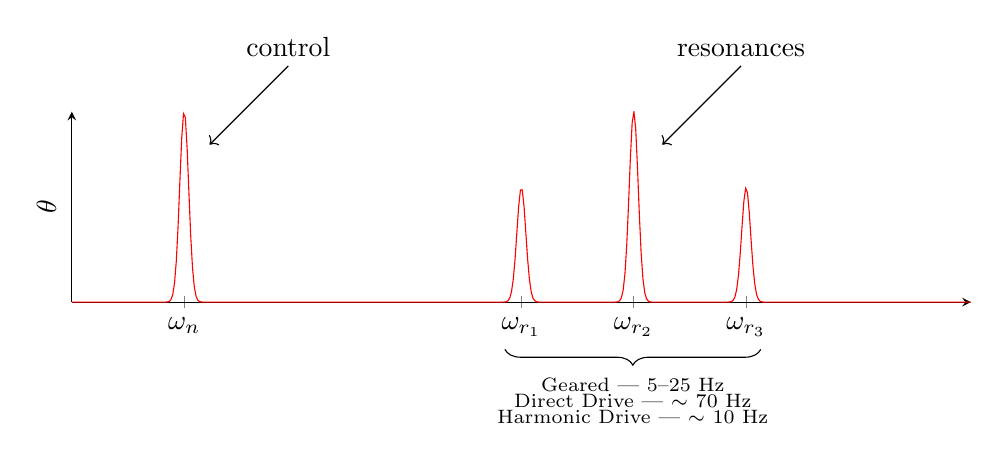
\begin{tikzpicture}
        \begin{axis}[
        		width=13cm,
		height=4cm,
            %ticks=none,
            axis lines = left,	
           % xlabel = $\omega$,
            ylabel = $\theta$,
            ytick=\empty,
            xtick={0.25, 1, 1.25, 1.5},
	    xticklabels={
    		$\omega_{n}$,
    		$\omega_{r_{1}}$,
		$\omega_{r_{2}}$,
    		$\omega_{r_{3}}$}
        ]
        \addplot[
        		color=red,
		domain=0:2,
		samples=500
	]
	{0.25*exp(-(x-0.25)^2/(2*0.01^2)) + 0.15*exp(-(x-1)^2/(2*0.01^2)) + 0.25*exp(-(x-1.25)^2/(2*0.01^2)) + 0.15*exp(-(x-1.5)^2/(2*0.01^2))};
        %\addplot[color=red, domain=0:1, samples=1000]{0.15*exp(-(x-1)^2/(2*0.01^2))};
        %\addplot[color=red, domain=0:1, samples=1000]{0.25*exp(-(x-1.25)^2/(2*0.01^2))};
        %\addplot[color=red, domain=0:1, samples=1000]{0.15*exp(-(x-1.5)^2/(2*0.01^2))};

        \end{axis}
        \draw[<-] (1.75, 2) -- (2.75, 3) node [above] {control};
        \draw[<-] (7.5, 2) -- (8.5, 3) node [above] {resonances};
	\draw[decoration={brace,amplitude=2mm,mirror,raise=1mm},decorate] (5.5, -0.5) -- (8.75, -0.5);
	\draw (7.125, -1.25) node {$\substack{\text{Geared --- 5--25 Hz}\\\text{Direct Drive --- $\sim$ 70 Hz}\\\text{Harmonic Drive ---  $\sim$ 10 Hz}}$};
    \end{tikzpicture}
\end{figure}

For the Ranger arm,
\begin{eqnarray}
	J_{m} & = & 0.00048\ \text{Kg--m}^{2} \nonumber \\
	J_{\text{link}} & = & 0.5\ \text{Kg--m}^{2} \nonumber \\
	\eta & = & 201 \nonumber \\
	\omega_{r} & = & \sqrt{\frac{K_{t}}{J_{\text{eff}}}} \nonumber \\
	J_{\text{eff}} & = & J_{\text{link}}+\eta^{2}J_{m} = 19.39+0.5 \nonumber \\
	\omega_{r} & = & 52.8\ \text{rad/sec} \nonumber \\
	\rightarrow f_{r} & = & 8.3\ \text{Hz} \nonumber
\end{eqnarray}

\subsection{Example 9.7 from the textbook}
Here's a spring--mass--damper system:
\begin{figure}[h!]
\centering
 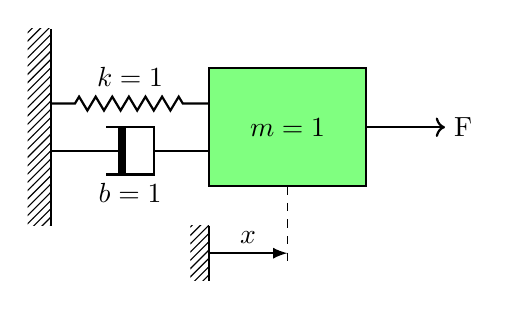
\begin{tikzpicture}[every node/.style={outer sep=0pt},thick,
 mass/.style={draw,thick},
 spring/.style={thick,decorate,decoration={zigzag,pre length=0.3cm,post
 length=0.3cm,segment length=6}},
 ground/.style={fill,pattern=north east lines,draw=none,minimum
 width=0.75cm,minimum height=0.3cm},
 dampic/.pic={\fill[white] (-0.1,-0.3) rectangle (0.3,0.3);
 \draw (-0.3,0.3) -| (0.3,-0.3) -- (-0.3,-0.3);
 \draw[line width=1mm] (-0.1,-0.3) -- (-0.1,0.3);}]

  \node[mass,minimum width=2cm,minimum height=1.5cm,fill=green!50] (m1) {$m=1$};
   \node[left=2cm of m1,ground,minimum width=3mm,minimum height=2.5cm] (g1){};
  \draw (g1.north east) -- (g1.south east);

  \draw[spring] ([yshift=3mm]g1.east) coordinate(aux)
   -- (m1.west|-aux) node[midway,above=1mm]{$k=1$};

  \draw ([yshift=-3mm]g1.east) coordinate(aux')
   -- (m1.west|-aux') pic[midway]{dampic} node[midway,below=3mm]{$b=1$};
 
 % \foreach \X in {1}  
  %\draw[thin] (m1.north) -- ++ (0,1) coordinate[midway](aux1);
   %\draw[latex-] (aux\X) -- ++ (-0.5,0) node[above]{$\tau$}; 
   \draw[thin,dashed] (m1.south) -- ++ (0,-1) coordinate[pos=0.85](aux'1);
   \draw[latex-] (aux'1) -- ++ (-1,0) node[midway,above]{$x$}
    node[left,ground,minimum height=7mm,minimum width=1mm] (g'1){};
   \draw[thick] (g'1.north east) -- (g'1.south east);
   \draw[->] (m1.east) -- ++ (1, 0) node [right] {F};
  %}

\end{tikzpicture}
\end{figure}

\noindent
and we are asked to find a decoupled joint controller such that $\zeta=1$, $K_{\text{tot}}=\text{MAX}$, and the controller does not excite any unmodelled dynamics (e.g. flexible modes).
 \noindent
So the dynamics are
\begin{displaymath}
	\ddot{x} + \dot{x} + x = F
\end{displaymath}
The controller will have the form
\begin{displaymath}
	F = \cancelto{0}{\ddot{x}_{d}} + (\dot{x}+x) - K_{v}\dot{x}-K_{p}x
\end{displaymath}
and the closed loop dynamics are
\begin{displaymath}
	\ddot{x}+K_{v}\dot{x}+K_{p}x=0
\end{displaymath}
We need to find $K_{p}$ and $K_{v}$:
\begin{eqnarray}
	K_{p} & = & \omega_{n}^{2} = \left(\frac{1}{2}\omega_{\text{res}}\right)^{2} = \left(\frac{1}{2}8\right)^{2} = 16 \nonumber \\
	K_{v} & = & 2\zeta\omega_{n} = 2(1)(4) = 8 \nonumber
\end{eqnarray}

\section{Friction}
Friction is a significant disturbance present in every robotic joint (and indeed, in every mechanism.) Friction is also a \emph{very} complex phenomenon that is very difficult to accurately model. We generally divide friction into at least three different types:

\begin{tblr}{
  colspec = {Q[m]Q[m]Q[m]},
  stretch = 0,
  rowsep = 6pt,
  hlines = {red5, 0pt},
  vlines = {red5, 0pt},
}
	&&\\
	Type & Equation & \parbox{2.2cm}{\centering Graph} \\
	&&\\
	Viscous, or wet & $F=-b_{v}\dot{x}$ &
	\parbox{4cm}{
	\begin{tikzpicture}
	        \begin{axis}[
	        	height=4cm,
		width=4cm,
	            ticks=none,
	            axis x line=center,
 		 axis y line=center,
		 enlarge y limits=0.2
	        ]
	        \addplot[
	        		color=red,
			domain=-0.5:0.5,
		]
		{-0.5*x};
	        \end{axis}
	       	\draw (2.75, 1.25) node {$\dot{x}$};
		\draw (1.25, 2.6) node {$F$};
        \end{tikzpicture}
        }
	\\
	Coloumb, or dry & $F=-b_{c}\text{sign}(\dot{x})$ &
		\parbox{4cm}{
		\begin{tikzpicture}
	        \begin{axis}[
	        	height=4cm,
		width=4cm,
	        ticks=none,
	        axis x line=center,
 		axis y line=center,
		enlarge y limits=0.2
	        ]
	        \addplot[
	        		color=red,
			domain=-1:1,
			samples=100
		]
		{-sign(x)};
	        \end{axis}
	        	\draw (2.75, 1.25) node {$\dot{x}$};
		\draw (1.25, 2.6) node {$F$};
        \end{tikzpicture}}
	\\
	Stiction & $F = \left\{ \begin{array}{cc} -F_{c} & \dot{x} = 0\text{ and }|F_{c}|<F_{s} \\ F_{z} & \text{ otherwise} \end{array} \right. $ &
		\parbox{4cm}{
		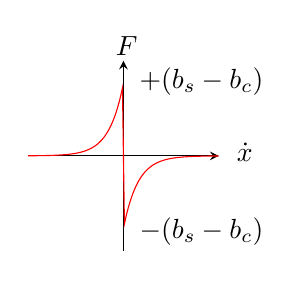
\begin{tikzpicture}
		\def\bc{0.25};
		\def\bs{1.25};
		\def\delt{0.15};
		\def\bv{0.75}
	        \begin{axis}[
	        	height=4cm,
		width=4cm,
	        ticks=none,
	        axis x line=center,
 		axis y line=center,
		enlarge y limits=0.2
	        ]
	        \addplot[
	        		color=red,
			domain=-1:1,
			samples=100
		]
		{-(\bs-\bc)*exp(-abs(x)/\delt)*sign(x)};
	        \end{axis}
	        \draw (2.2, 0.25) node {$-(b_{s}-b_{c})$};
	        \draw (2.2, 2.15) node {$+(b_{s}-b_{c})$};
	        \draw (2.75, 1.25) node {$\dot{x}$};
		\draw (1.25, 2.6) node {$F$};
        \end{tikzpicture}}
 	\\
	& $F_{z} = -(b_{s}-b_{c})e^{-(|\dot{x}|/\delta)}\text{sign}(\dot{x})  $ & \\
\end{tblr}
\vspace{0.5cm}

\noindent
where the parameters in the stiction model are $b_{s}$, the static coefficient of friction; $F_{c}$ is the nominal control input to the joint, and $\delta$ is the ``Stribeck velocity'', below which the joint is in the stick--slip regime. Note that this model is an attempt to model stiction deterministically, but actual stick--slip is nearly impossible to model except probabilistically, in the sense when operating the joint near the Stribeck velocity the actual force or torque needed to ``break'' away from a stick phenomenon and transition to a slip phenomenon is randomly distributed around $F_{c}$, as is the distance over which the joint will ``slip'' before entering a ``stick'' regime again. In addition, stick--slip can change quite dramatically with joint load. Stick--slip can be particularly challenging when using compliance control because in most cases, tasks requiring compliance require low Cartesian velocities along most, if not all, axes, so you are almost always operating below the Stribeck velocity. This leads to what appears to be ``hunting'' behavior.

There are many more complex models of friction, and particularly stiction. The model we have used here is from Márton and Lantos, ``Control of mechanical systems with Stribeck friction and backlash,'' Systems \& Control Letters 58.2 (2009), pp. 141-147. For more information on friction models a good reference is Waiboer, Aarts, and Jonker, ``Velocity dependence of joint friction in robotic manipulators with gear transmissions,'' ECCOMAS Thematic Conference Multibody Dynamics (2005).

\noindent
Adding all of these together, we get a decent model for the total friction known as a Stribeck curve:
\begin{figure}[h!]
\centering
\begin{tikzpicture}
%		\def\bc{-0.25};
%		\def\bs{-1.25};
%		\def\delt{-0.75};
%		\def\vs{5};
		\def\bc{0.25};
		\def\bs{1.25};
		\def\delt{0.15};
		\def\bv{0.75}
	        \begin{axis}[
	        	height=6cm,
		width=12cm,
	        ticks=none,
	        axis x line=center,
 		axis y line=center,
		enlarge y limits=0.2
	        ]
	        \addplot[
	        		color=red,
			domain=-2:2,
			samples=200
			]
			%{(\fc + \fs*exp(-\vs*abs(x)))*sign(x)+\fv*x} coordinate [pos=0.77] (C) coordinate [pos=0.85] (A) coordinate [pos=0.9] (B);
			%{-\bc*sign(x) + (\bs-\bc)*exp(-((x/\delt)^2))*-sign(x) -\bv*x} coordinate [pos=0.77] (C) coordinate [pos=0.85] (A) coordinate [pos=0.9] (B);
			{-\bc*sign(x) - (\bs-\bc)*exp(-abs(x)/\delt)*sign(x) - \bv*x} coordinate [pos=0.74] (C) coordinate [pos=0.85] (A) coordinate [pos=0.9] (B);
	        \addplot[
	        		color=red!70,
			domain=0:1,
			dashed,
			samples=100
			]
			{(-\bc*sign(x)-\bv*x};
			\draw (A) -| (B);
			\draw ($(B)+(15, 15)$) node {$-b\dot{x}$};
			%\newdimen\X;
			%\newdimen\Y;
			\draw[dashed] let \p1=(C), \p2=(current axis.origin) in (C) -- (\x1, \y2) node[above] {$\delta$};
	        \end{axis}
%		\path (C); \pgfgetlastxy{\X}{\Y};
%		\draw (C) -- (axis cs:\X, 0);
		\draw[decorate,decoration={brace,amplitude=10pt,mirror,raise=2pt},yshift=0pt] (current axis.origin) -- ($(current axis.origin)+(0, -\bc)$) node [black,midway,xshift=-0.8cm] {$-b_{c}$};
		\draw[decorate,decoration={brace,amplitude=10pt,mirror,raise=2pt},yshift=0pt] ($(current axis.origin)+(0, -\bc)$) -- ($(current axis.origin)+(0, -\bs)$) node [black,midway,xshift=-0.8cm] {$-b_{s}$};
		\node [right] at (current axis.right of origin) {$\dot{x}$};
		\node [above] at (current axis.above origin) {$F$};
\end{tikzpicture}
\end{figure}

\noindent
where the mathematical model is
\begin{displaymath}
	F = -b_{c}\text{sign}(\dot{x}) -(b_{s}-b_{c})e^{-(|\dot{x}|/\delta)}\text{sign}(\dot{x}) - b\dot{x}
\end{displaymath}

\section{Backlash}
Backlash refers to the ``slop'' in a gear train where one of the two gears moves before engaging the other gear. Backlash on the inside of a control loop (e.g. where you are measuring the output side of the geartrain) leads to limit cycles. Backlash on the outside of a control loop, where you are measuring the input side of the geartrain, leads to position errors. There is a strict tradeoff between backlash, friction, and compliance. Harmonic gears, for instance, tend to have low backlash but high friction and compliance. Planetary gears tend to have higher backlash but lower friction and compliance.
\begin{figure}[h!]\centering
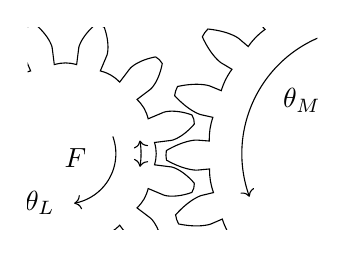
\begin{tikzpicture}[scale=0.08]
		\clip (-6,-12) rectangle (40,20);
		\gear{3}{12}{20}
		\begin{scope}[xshift=49cm,rotate=180/19]
			\gear{3}{20}{20}
		\end{scope}
		\draw[->] ([shift={(0cm,0cm)}]20:8) arc [start angle=20, end angle=-80, radius=8cm] node[near start, left=0.25cm] {$F$} node[left=0.125cm] {$\theta_{L}$};
		\draw[<->] ([shift={(0cm,0cm)}]10:12) arc [start angle=10, end angle=-10, radius=12cm];
		\draw[->] ([shift={(48cm,0cm)}]110:20) arc [start angle=110, end angle=200, radius=20cm] node[midway, right=0.25cm] {$\theta_{M}$};
\end{tikzpicture}
\end{figure}
\end{document}
